\documentclass[conference]{IEEEtran}
\IEEEoverridecommandlockouts
% The preceding line is only needed to identify funding in the first footnote. If that is unneeded, please comment it out.
\usepackage{cite}
\usepackage{amsmath,amssymb,amsfonts}
\usepackage{algorithmic}
\usepackage{graphicx}
\usepackage{textcomp}
\usepackage{xcolor}
\usepackage{caption}


\def\BibTeX{{\rm B\kern-.05em{\sc i\kern-.025em b}\kern-.08em
    T\kern-.1667em\lower.7ex\hbox{E}\kern-.125emX}}
\begin{document}

\pagestyle{plain}

\title{DAL 2023 - Assignment 2\\
{\footnotesize}

}

\author{\IEEEauthorblockN{Pranoy K P}
\IEEEauthorblockA{\textit{Engineering Design} \\
\textit{Indian Institute of Technology Madras}\\
\textit{ed20b045@smail.iitm.ac.in}
}
}

\maketitle

\begin{abstract}
In this study, we tackle the challenge of predicting survival outcomes for passengers aboard the RMS Titanic during its ill-fated maiden voyage in 1912. Leveraging the provided datasets, we aim to discern factors influencing passenger survival, such as age, gender, socioeconomic class, etc. With the training dataset providing the ground truth for 891 passengers, we employ machine learning techniques to build a predictive model. This research aims to shed light on the dynamics of survival during maritime disasters and contribute to our understanding of the Titanic tragedy’s enduring impact.
\end{abstract}
\vspace{1mm} %vertical space

\section{INTRODUCTION}

In this paper, we employ logistic regression to explore the correlation between the survival rates of Titanic passengers and various factors such as age, gender, socioeconomic status, and more. This analysis aims to provide insights into potential biases that may have influenced survival outcomes during that era. 

Logistic regression addresses classification problems by calculating probabilities based on input characteristics. In binary classification, a threshold is established, and items are categorised into one class if the probability exceeds this threshold and into another class if it falls below it. 

Our dataset comprises passenger information from the RMS Titanic, encompassing details like name, age, gender, socioeconomic status, social class, and additional data such as the number of siblings, ticket information, cabin number, and port of embarkation. The training dataset includes valuable information about the passengers who survived the disaster, which we use to construct a predictive model for assessing a passenger’s likelihood of survival in the test dataset. Throughout the paper, we delve into the fundamental principles of logistic regression and apply this technique to predict the survival probabilities of passengers based on a set of input features.

The paper aims to study the concepts behind logistic regression and leverage it to delve into the Titanic passenger dataset. We then use this technique to predict the passengers’ survival probability from the given set of input features. By modelling the survival probabilities, we can better understand the tragic events surrounding the Titanic disaster.

\vspace{2mm} %vertical space

\section{LOGISTIC REGRESSION}

\subsection{Definition}
Logistic regression is a supervised machine learning algorithm used to tackle classification problems. Logistic regression models a relationship between predictor variables and a categorical response variable. The different types of logistic regression, depending on the nature of the categorical response, are:

\begin{enumerate}
    \item \textbf{Binary Logistic Regression:} Used when the response is binary (two possible outcomes). 
    \item \textbf{Nominal/Multiclass Logistic Regression:} Used when three or more classes exist.
\end{enumerate}

The logistic regression model converts the continuous output from the linear regression function into a categorical output by employing a sigmoid function. This sigmoid function, or the logistic function, takes any set of real-valued independent variables as input and maps them to a value from 0 to 1.

\[ z(x) = w^Tx + b \]

Here, x represents the input matrix, w is the weights or coefficient matrix, and b is the bias term, also known as intercept.

\[ \sigma(z) = \frac{1}{1 + e^{-z}} \]

Now, we use the sigmoid function where the input will be z and find the probability between 0 and 1.

\begin{figure}[htbp]
\centerline{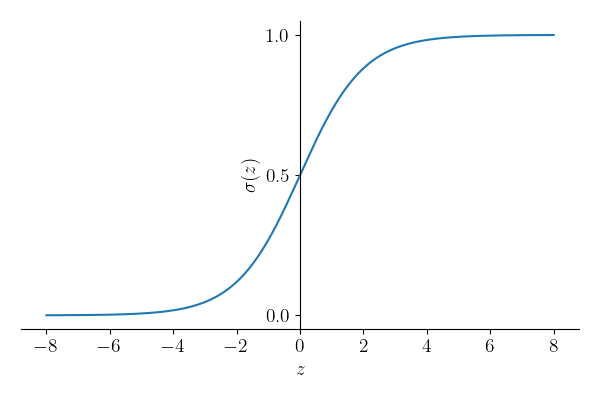
\includegraphics[scale = 0.6]{logistic regression.png}}
\caption{Sigmoid Function}
\label{fig}
\end{figure}

Consider two classes, A and B, for our binary classification problem. The classification rule is as follows:

\begin{align*}
\text{if } p < \text{Threshold}, & \quad \hat{y} = A \\
\text{if } p \geq \text{Threshold}, & \quad \hat{y} = B
\end{align*}

\subsection{Cost Function}
The cost function measures the performance of a machine learning model for a data set. The cost function quantifies the error between predicted and expected values and presents that error as a single real number. The cost function employed is Log Loss or Cross Entropy. It is defined as:
\[
J(\theta) = -\frac{1}{m} \sum_{i=1}^{m} \left[y_i\log(h_\theta(x_i)) + (1 - y_i)\log(1 - h_\theta(x_i))\right]
\]

\begin{figure}[htbp]
\centerline{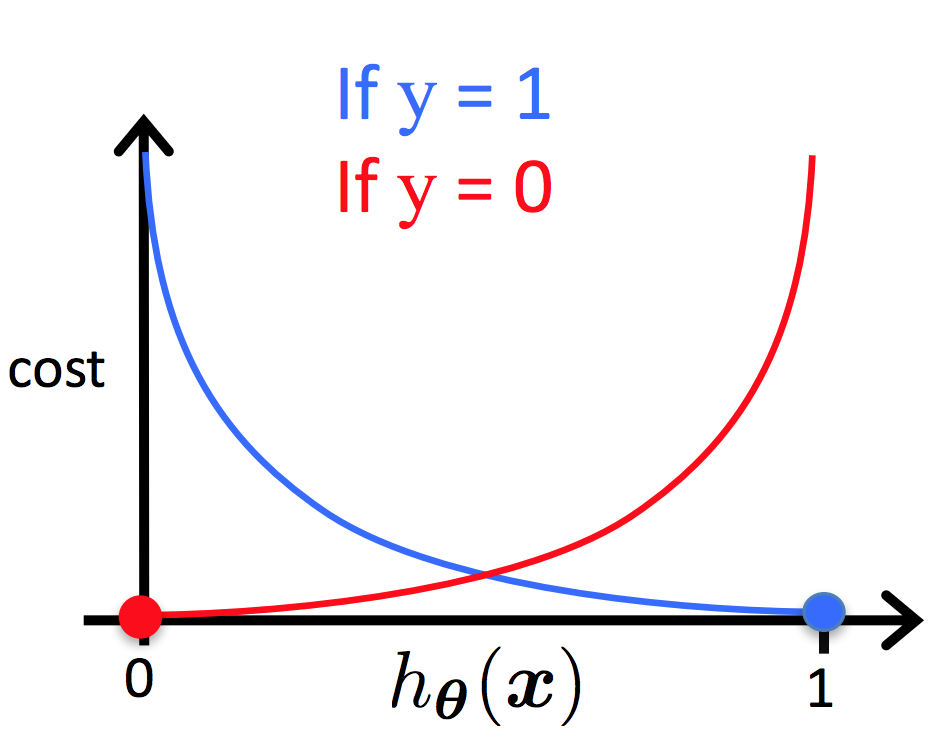
\includegraphics[scale = 0.5]{cost function.png}}
\caption{Cost Function}
\label{fig}
\end{figure}

\subsection{Gradient Descent}
Gradient Descent is one of the most commonly used optimisation algorithms to train machine learning models by minimising errors between actual and expected results. The gradient points in the direction of the steepest increase in the function, and moving in the opposite direction leads to the most significant reduction in the cost. During each iteration, we reduce the cost moving along this direction, and the size of each step is determined by the hyperparameter known as the learning rate \(\alpha\). This iterative process continues until a stopping criterion is met.

The choice of the learning rate is crucial. If it’s too small, it would require excessive iterations to converge. Similarly, the output can oscillate and diverge from the optimal solution if it’s too large. Therefore, finding an appropriate learning rate is crucial to gradient descent optimisation.

\vspace{2mm} %vertical space

\section{THE PROBLEM}
This section will apply the earlier mathematical principles to conduct our data analysis. Our objective is to assess the influence of all the variables within the Titanic dataset and make an attempt to estimate the likelihood of passengers’ survival in the test dataset.

\subsection{Imputation for Missing Values}
\begin{enumerate}
    \item {Port of Embarkation:} As depicted in the bar chart in Fig. 3, it’s evident that the majority of passengers boarded from Southampton. So, we have chosen to fill in all the missing values with Southampton as the port of embarkation. 
    \begin{figure}[htbp]
    \centerline{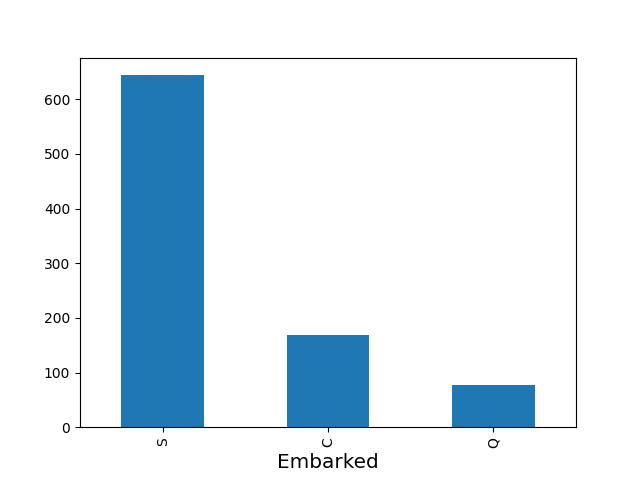
\includegraphics[scale = 0.56]{port_histogram.png}}
    \caption{Port of Embarkation}
    \label{fig}
    \end{figure}
    \item {Age:} Fig. 4 reveals that the distribution of ages is not uniform. We employ a strategy based on passenger titles extracted from the name column to address missing age values. We compute the mean age for each title and use this information to impute the missing ages for passengers accordingly.
    \begin{figure}[htbp]
    \centerline{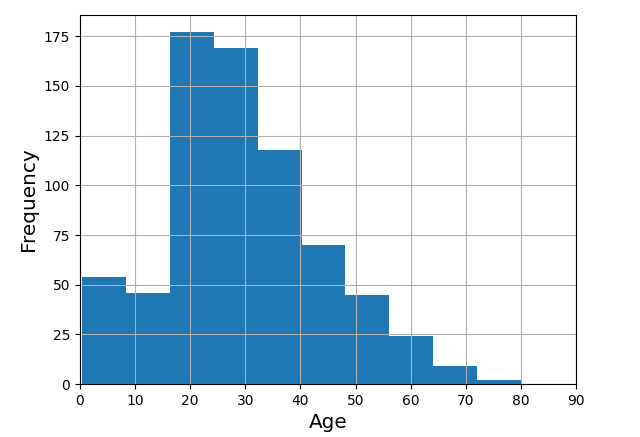
\includegraphics[scale = 0.56]{age_histogram.png}}
    \caption{Age Distribution}
    \label{fig}
    \end{figure}
\end{enumerate}

\subsection{Exploratory Data Analysis}
This is a crucial step in understanding the data before building a logistic regression or any other machine learning model. EDA helps you gain insights into your dataset, identify patterns, detect anomalies, and make informed decisions about data preprocessing and feature selection. 
\begin{enumerate}
    \item Fare vs. Survival: Drawing from the information presented in Figure 5, it is evident that a higher fare substantially increased the likelihood of survival. The dataset highlights a significant portion of individuals with lower fares who, unfortunately, did not survive. This might shed light on the hierarchy of social classes. As indicated by the fare class, socioeconomic status played a notable role in determining survival outcomes during the Titanic’s unfortunate event.
    \begin{figure}[htbp]
    \centerline{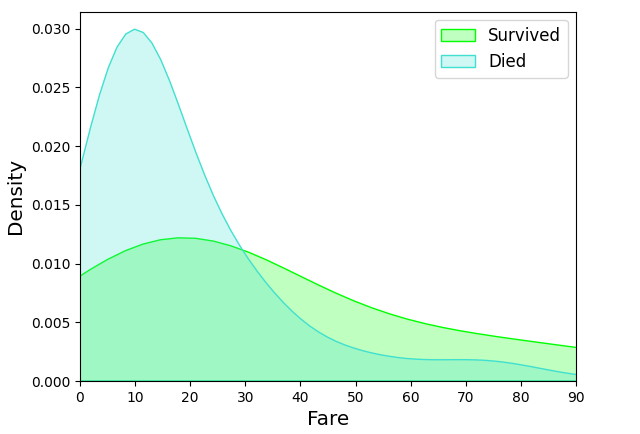
\includegraphics[scale = 0.56]{Fare versus Survival.png}}
    \caption{Fare vs Survival}
    \label{fig}
    \end{figure}
    \item Age vs. Survival: The plot in Fig. 6 highlights that children received preferential treatment during the rescue operations. This makes sense because the lives of innocent children would have been put above the lives of adults.
    \begin{figure}[htbp]
    \centerline{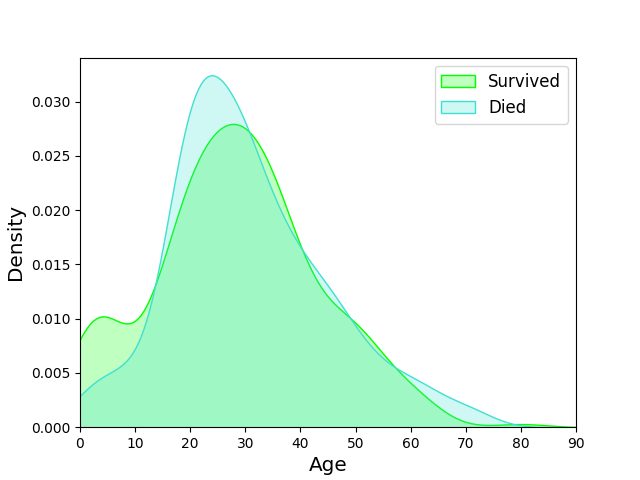
\includegraphics[scale = 0.56]{Age versus Survival.png}}
    \caption{Age vs Survival}
    \label{fig}
    \end{figure}
    \item Passenger Class vs. Survival: By examining the bar plot in Figure 7, it becomes apparent that passengers in the first-class category had a higher probability of surviving the rescue operation. This suggests that choosing the third class was associated with a higher level of risk during the journey.
    \begin{figure}[htbp]
    \centerline{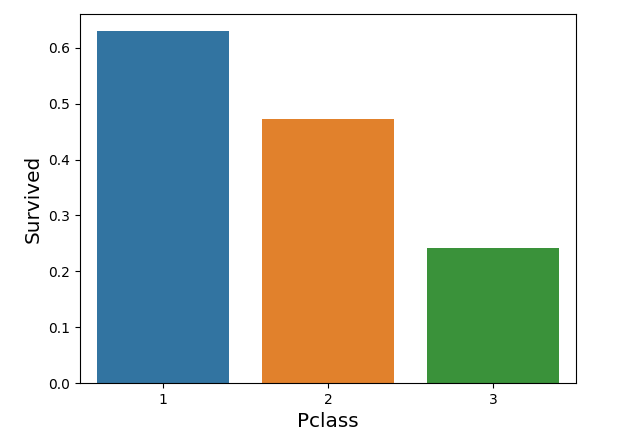
\includegraphics[scale = 0.56]{Passenger Class versus Survival.png}}
    \caption{Passenger Class vs Survival}
    \label{fig}
    \end{figure}
    \item Port of Embarkation vs. Survival: As indicated by Figure 8, passengers who embarked from Cherbourg displayed the highest survival rate compared to passengers from the other two ports. This relationship corresponds with the observation that Cherbourg passengers had the highest average fare, amounting to 59.95 (as shown in Table 1). This suggests that the more affluent demographic who boarded from Cherbourg were more likely to survive the tragedy.
    \begin{figure}[htbp]
    \centerline{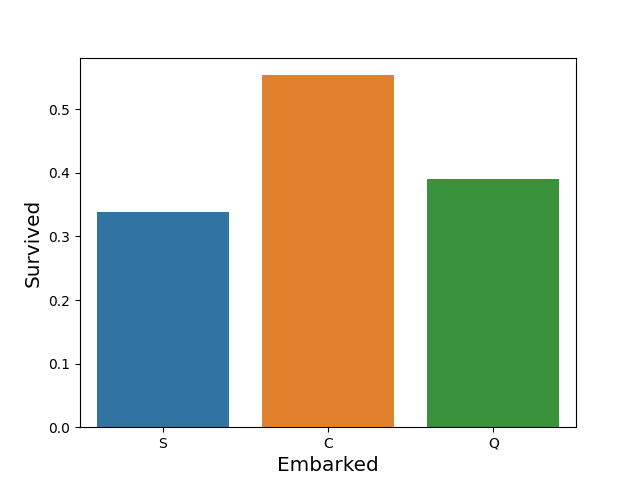
\includegraphics[scale = 0.56]{Port of Embarkation versus Survival.png}}
    \caption{Port of Embarkation vs Survival}
    \label{fig}
    \end{figure}
    \begin{table}[h!]
      \begin{center}
        \caption{{Mean Fare and Survival Rate of Passengers}}
        \label{tab:table1}
        \renewcommand{\arraystretch}{1.2} % Adjust cell height
        \begin{tabular}{c|c|c} % <-- Alignments: 1st column left, 2nd middle and 3rd right, with vertical lines in between
          \textbf{Embarked} & \textbf{Fare} & \textbf{Survival Rate}\\
          \hline
          C & 59.954 & 0.554 \\
          Q & 13.276 & 0.390 \\
          S & 27.080 & 0.337 \\
        \end{tabular}
      \end{center}
    \end{table}

    \item Sex vs. Survival: As indicated in Fig. 9, females had a considerably higher chance of survival than males. This can be attributed to the historical practice of prioritising women and children during emergencies. This courteous approach led to a notably higher survival rate among female passengers than their male counterparts.
    \begin{figure}[htbp]
    \centerline{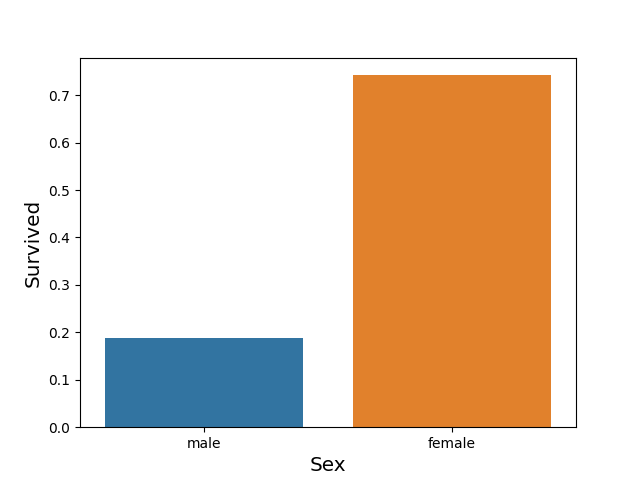
\includegraphics[scale = 0.56]{ Sex versus Survival.png}}
    \caption{Sex vs Survival}
    \label{fig}
    \end{figure}
    \item Family size vs Survival: The data suggests that passengers travelling in groups had a notably higher likelihood of survival than those travelling alone. 
    \begin{table}[h!]
      \begin{center}
        \caption{{Family Size vs Survival}}
        \label{tab:table1}
        \renewcommand{\arraystretch}{1.2} % Adjust cell height
        \begin{tabular}{c|c} 
          \textbf{Size} & \textbf{Survived}\\
          \hline
          Groups & 0.505650\\
          Alone & 0.303538\\
        \end{tabular}
      \end{center}
    \end{table}
\end{enumerate}

\subsection{Feature Engineering}
\begin{enumerate}
    \item Titles: During the tragedy, a person’s titles indicated their rank and societal status, factors that played a role in the rescue efforts. Consequently, we incorporate this aspect into our model.
    
    \item Family Size: Utilising data on the number of siblings, parents, and children, we estimate the family size for each passenger. To account for this, we introduce a separate column labelled ‘Alone’ to track whether a passenger was travelling alone or with companions. We realise that group travellers are more likely to survive than solo passengers. We incorporate this information into our model.
    
    \item Column Removal: We eliminate the ‘SibSp’ and ‘Parch’ columns since we have extracted valuable information from them. Additionally, we drop the ‘Cabin’ and ‘Ticket’ columns as they contribute very little to our analysis.
\end{enumerate}

\subsection{Model Fitting}
Following data cleaning, preprocessing, and feature engineering, we employed the sklearn library to train a logistic regression model on the refined training dataset. The training accuracy of the model stands at 81.59\%. To gain a deeper insight into our model’s performance, we constructed a confusion matrix presented in Table 3 above.

\begin{table}[h!]
  \centering
  \caption{Confusion Matrix for Logistic Regression Model}
  \label{tab:table}
  \begin{tabular}{|c|c|c|}
    \hline
    \textbf{} & \textbf{Positive (Actual)} & \textbf{Negative (Actual)} \\
    \hline
    \textbf{Positive (Prediction)} & 476 & 73 \\
    \hline
    \textbf{Negative (Prediction)} & 91 & 251 \\
    \hline
  \end{tabular}
\end{table}

\vspace{2mm} %vertical space

\section{CONCLUSIONS}
In this study, we applied logistic regression techniques to real-world data, and the outcomes illustrate the applicability of logistic regression to complex, real-world datasets. Based on our analysis, it can be inferred that factors such as societal status, income, ticket class, gender, and family roles all influenced passengers’ survival rates during the Titanic disaster. This leads us to question how different segments of the affluent population were impacted and whether certain benefits and incentives persisted.

\begin{thebibliography}{10}
\bibitem{b1}Aurelian Geron, Hands-On Machine Learning with Scikit-Learn, Keras, and TensorFlow: Concepts, Tools and Techniques to Build Intelligent Systems, O’Reilly Media, Inc., pp. 33–143
\bibitem{b2}Bishop Christopher M.. 2006. Pattern Recognition and Machine Learning. Springer. pp.179-224.
\end{thebibliography}
\vspace{12pt}

\end{document}